\section{Imágenes y píxeles}

 Una imagen es un tipo de dato discreto que representa una realidad observada en una matriz. En cada posición, se le asigna una representación del color. Estas posiciones podrían tener un valor único en el caso de las imágenes en blanco y negro, o tres valores en caso de las imágenes a color, usualmente RGB (rojo, verde y azul).

Para representar una imagen en términos de la matemática, la consideramos una función $I : \Omega \subset \mathbb{Z}^2 \to \mathbb{R}^c$ tal que mapea coordenadas espaciales $(x,y)$ a valores de intensidad para cada uno de los $c$ canales. Cada canal representa una componente del color, estando los valores en el intervalo $[0,1]$ o en el intervalo de enteros entre $0$ y $255$. El modelo computacional más común es el de una matriz, donde, en orden, se guarda el valor de intensidad de cada píxel en cada canal. En algunos casos, resulta conveniente utilizar una matriz por canal, es decir, teniendo $c$ funciones que devuelven escalares, en lugar de una única función que devuelve un vector de tamaño $c$.

Cada posición de la matriz se conoce como píxel, (del inglés \textit{picture element}). Aunque se los visualiza con frecuencia como cuadrados de colores, los píxeles son muestras puntuales de la realidad, que es continua. Esto nos lleva a que una imagen es una grilla de puntos con espacios vacíos entre ellos. Para no tener esos espacios vacíos, una forma de rellenarlos es usar la información de los píxeles más cercanos para estimar un posible valor para cada punto no muestreado del espacio. A partir del teorema de muestreo de Nyquist-Shannon, sabemos que se puede reconstruir una entidad continua a partir de una discreta usando un filtro de reconstrucción \cite{SmithPixel} bajo ciertas condiciones. En la práctica, los algoritmos de visión por computadora trabajan directamente sobre las imágenes obtenidas por la cámara, pero se fundamentan en la idea de trabajar sobre muestras.

El tamaño de la muestra tomada en la imagen se conoce como resolución, expresada como la cantidad de píxeles en cada dimensión. Por ejemplo, una imagen de $1920 \times 1080$ tiene $1920$ píxeles en la coordenada horizontal y $1080$ en la vertical. La resolución afecta la cantidad de detalles que se pueden capturar en la imagen, así como el tamaño del archivo y el tiempo de procesamiento necesario para analizarla. Por ello, es importante elegir una resolución adecuada, siendo que una resolución alta es más costosa pero trae consigo más información. Cuando la resolución de la imagen es demasiado alta para el procesamiento, se aplican técnicas de muestreo para reducir la resolución, conocidas como \textit{downsampling} o submuestreo.

\begin{figure}[H]
    \centering
    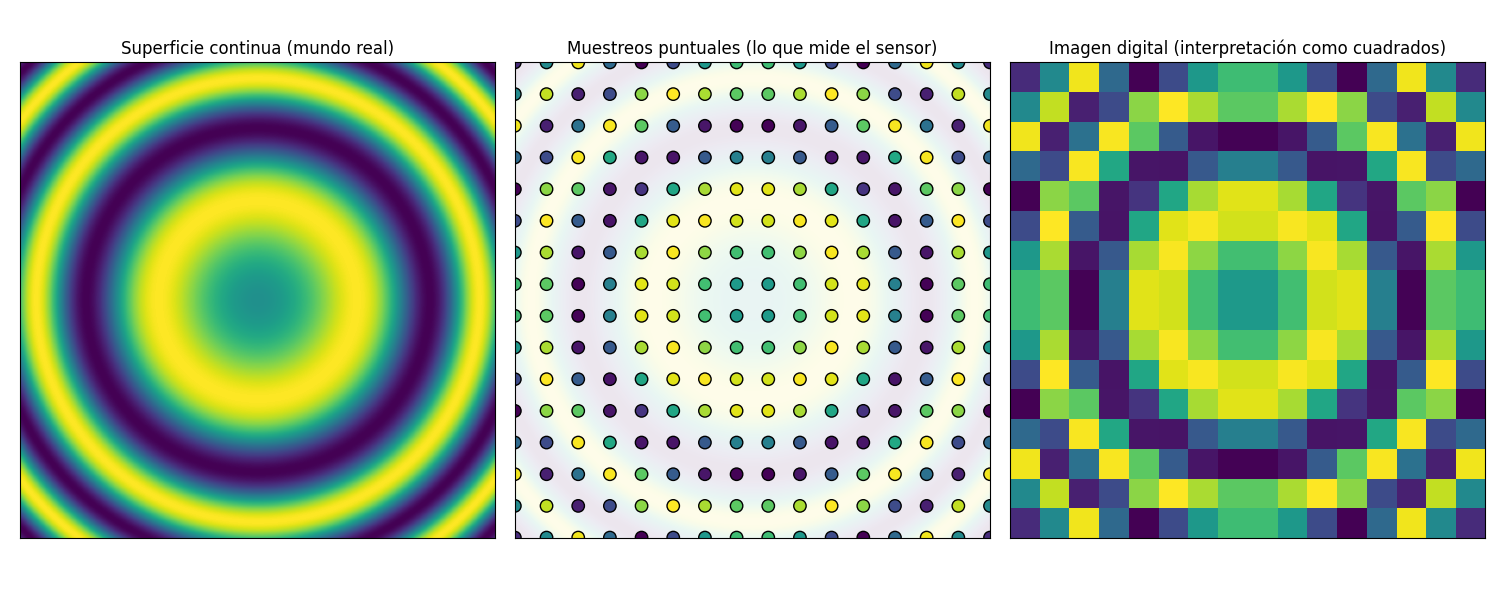
\includegraphics[width=0.7\linewidth, trim = 0cm 0cm 0cm 1.5cm, clip]{../imagenes_marco_teorico/pixel_que_es.png}
    \caption{Se observa a la izquierda una superficie, a la cual se le toma un muestreo en forma de grilla en el centro. Estos puntos son los que se conocen como píxeles. A la derecha, se muestra qué sucede si se interpretan los píxeles como cuadrados, que es la forma usual en la que se observan en computadora.}
    \label{fig:modelo_de_pixel}
\end{figure}